\documentclass[aspectratio=169]{beamer}
\usepackage[utf8]{inputenc}
\usepackage{amsmath}
\usepackage{amsfonts}
\usepackage{hyperref}
\usepackage{graphicx}
\usepackage{fontspec}
\usepackage{glossaries}
\usepackage{xcolor}
\usepackage{fontspec}
\usepackage{minted}

\definecolor{cblak}{RGB}{35,35,35} 
\usemintedstyle{solarized-dark}
%\usemintedstyle{tango}

\renewcommand\mathfamilydefault{\rmdefault}
\newcommand{\curdir}{.}


\newfontfamily\Nepali[Scale=1.1,Script=Devanagari]{Laila}
\newcommand{\Devanagari}[1]{{\Nepali #1}}
\newcommand{\code}[2][python]{\mintinline[fontsize=\footnotesize]{#1}|#2|}

\usetheme{CambridgeUS}

\useinnertheme{rectangles}

\input{DarkColour.tex}

%\usefonttheme{professionalfonts} %mkes math fonts original

%\newcommand{\code}[2][python]{\mintinline{#2}|#1|}
\author{Prakash Gautam \\ \Nepali{[ प्रकाश गौतम ]}}
\title{Speeding up \LaTeX}

%\setbeamercovered{transparent}

\date{\today} 
\subject{Physics} 

\begin{document}

\titlepage
%\phantom{\gls{tpc} \gls{roi} \gls{pdf}}\vspace*{-1cm}

%\begin{frame} \frametitle{Outline}
%\tableofcontents
%\end{frame}
\renewcommand{\bf}[1]{\textcolor{red!60}{#1}}

\section{परिचय}
%
%
\begin{frame}{Random}
     \begin{columns}
        \begin{column}{0.49\textwidth}
            \begin{itemize}
                \item Tiny Mountainous Country, area comparable to PA
                \item Our language is Nepali, written in Devangari Script, {\Nepali देवनागरी लिपी}
            \end{itemize}
            %\begin{block}{Hey I am here}
            %    And this is it.  
            %\end{block}
        \end{column}
        \begin{column}{0.49\textwidth}
            \begin{figure}[h!]
                \centering
                \only<1>{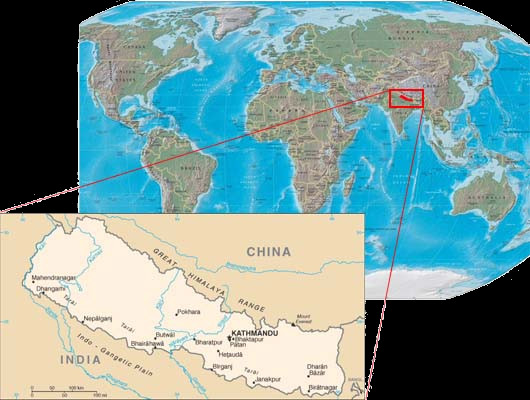
\includegraphics[width=\linewidth]{images/NepalZoomed_dark.jpeg}}
            \end{figure}
            %
        \end{column}
    \end{columns}
\end{frame} 
%
%
%\titlepage
%
\section{Introduction}
%
\begin{frame}{\LaTeX}
    \begin{columns}
        \begin{column}{0.49\textwidth}
            \begin{itemize}
                \item \LaTeX %(/ˈlɑːtɛx/ LAH-tekh or /ˈleɪtɛx/ LAY-tekh) %
                    is a document preparation system
                \item \TeX is the typesetting engine, 
                    \begin{itemize}
                        \item Low level macros, very hard to remember and write
                    \end{itemize}
                \item \LaTeX is layer over \TeX which is widely used
                \item Various variants of these available, pdfLatex, luaLatex, xeLatex, conTex
                \item Multiple distributions for different architecture, Tex-Live, MikTex, etc
            \end{itemize}
        \end{column}
        \begin{column}{0.49\textwidth}
            \begin{figure}[h!]
                \centering
                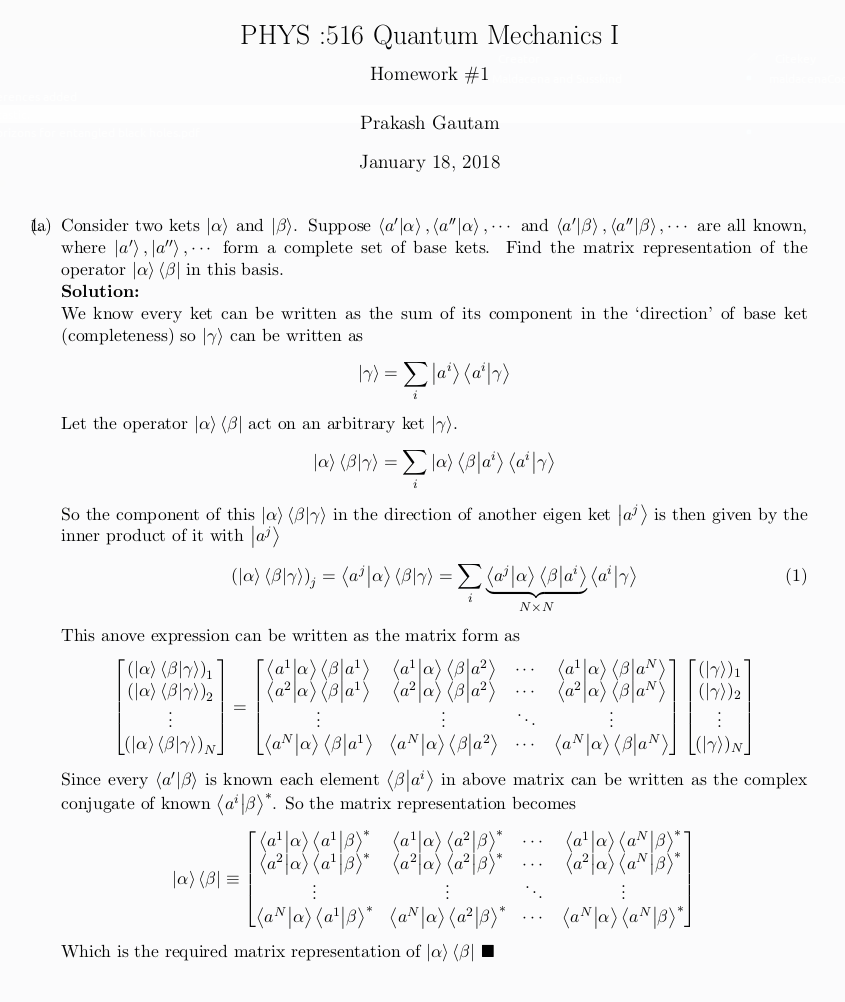
\includegraphics[width=0.8\linewidth]{images/QHW1_light.png}
                %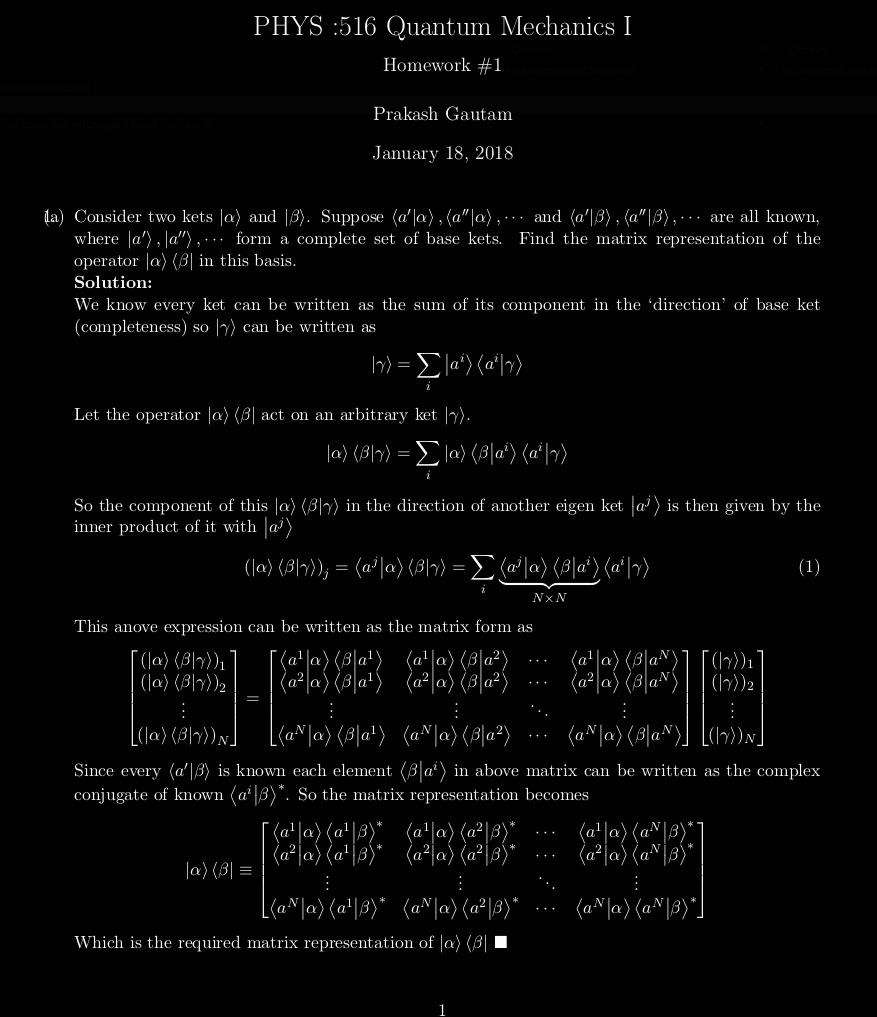
\includegraphics[width=0.8\linewidth]{images/Dark.png}
            \end{figure}
        \end{column}
    \end{columns}
\end{frame} 
%
%
\begin{frame}{Compilation}
    \begin{columns}
        \begin{column}{0.39\textwidth}
            \begin{itemize}
                \item \code{lualatex <source_file.tex>}
                \item \code{latexmk} is a useful tool, which handles
                    \begin{itemize}
                        \item multiple compilations 
                        \item missing cross references
                    \end{itemize}
                \item \code{latexmk <cource_file.tex>}
            \end{itemize}
        \end{column}
        \begin{column}{0.59\textwidth}
            \begin{columns}
                \begin{column}{0.49\textwidth}
                    \code[text]{~/.latexmkrc}\\
                    \inputminted[fontsize=\tiny,bgcolor=cblak,breaklines=true]{bash}{latexmkrc}
                \end{column}
                \begin{column}{0.49\textwidth}
                    \inputminted[fontsize=\tiny,bgcolor=cblak]{bash}{latextree.tex}
                \end{column}
            \end{columns}
        \end{column}
    \end{columns}
\end{frame} 
%
%
\section{Speeding Up}
%

%
\begin{frame}{Basics}
    \begin{columns}
        \begin{column}{0.39\textwidth}
            \begin{itemize}
                \item<1-> A good and customizable text editor is very essential
                \item<1-> Using syntax highlighting
                \item<1-> Using proper indentation
                \item<1-> Code folding makes it a lot easier.
            \end{itemize}
        \end{column}
        \begin{column}{0.59\textwidth}
            \begin{columns}
                \begin{column}{0.49\textwidth}
                    \only<1>{\inputminted[fontsize=\Tiny,bgcolor=cblak]{text}{noindent.tex}}
                \end{column}
                \begin{column}{0.49\textwidth}
                    \only<1>{\inputminted[fontsize=\Tiny,bgcolor=cblak]{latex}{styuse.tex}}
                \end{column}
            \end{columns}
        \end{column}
    \end{columns}
\end{frame} 
%
%
%
\begin{frame}{File Organization}
    \begin{columns}
        \begin{column}{0.39\textwidth}
            \begin{itemize}
                \item<1-> Break large file into multiple small files.
                \item<1-> Use \mintinline{latex}| \input{file.tex}|.
                \item<2-> Use \code{~/texmf} directory for common repeated files.
            \end{itemize}
        \end{column}
        \begin{column}{0.59\textwidth}
            \begin{columns}
                \begin{column}{0.49\textwidth}
                    \only<1>{\inputminted[fontsize=\tiny,bgcolor=cblak]{latex}{thesis.tex}}
                    \only<2>{\inputminted[fontsize=\tiny,bgcolor=cblak,breaklines=true]{latex}{usetexmf.txt}}
                \end{column}
                \begin{column}{0.49\textwidth}
                    \only<1>{\inputminted[fontsize=\tiny,bgcolor=cblak]{latex}{breakfiles.txt}}
                    \only<2>{\inputminted[fontsize=\Tiny,bgcolor=cblak]{latex}{texmftree.txt}}
                \end{column}
            \end{columns}
        \end{column}
    \end{columns}
\end{frame} 
%
%
%
%
\begin{frame}{Character Heatmap (aka Fancy 1D histogram)}
    \begin{columns}
        \begin{column}{0.49\textwidth}
            \begin{itemize}
                \item Character heatmap shows the relative frequency of characters in a text file over keyboard image
                \item Apply gaussian smoothing for nicer look.
                \item Take a \texttt{.tex} source file generate heatmap
                \item Compile \texttt{.tex} to \texttt{.pdf} > extract text from pdf > Generate Heatmap
            \end{itemize}
        \end{column}
        \begin{column}{0.49\textwidth}
            \begin{figure}[h!]
                \centering
                \only<1>{\mintinline{text}|text_heavy.tex| file \\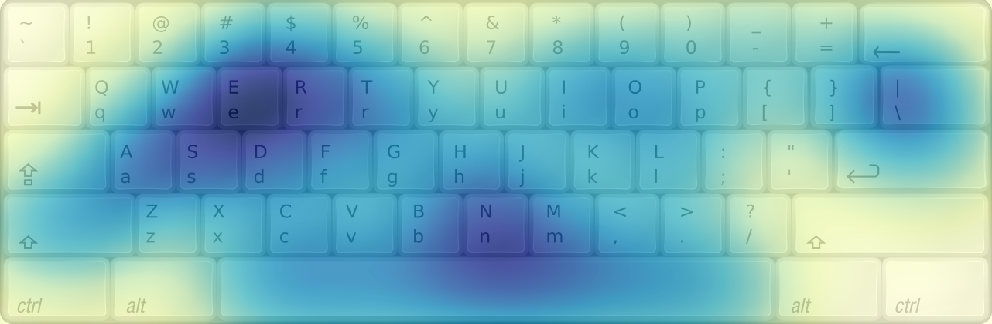
\includegraphics[width=\linewidth]{images/NoMathTex.png}}
                \only<1>{\mintinline{text}|text_heavy.txt| file \\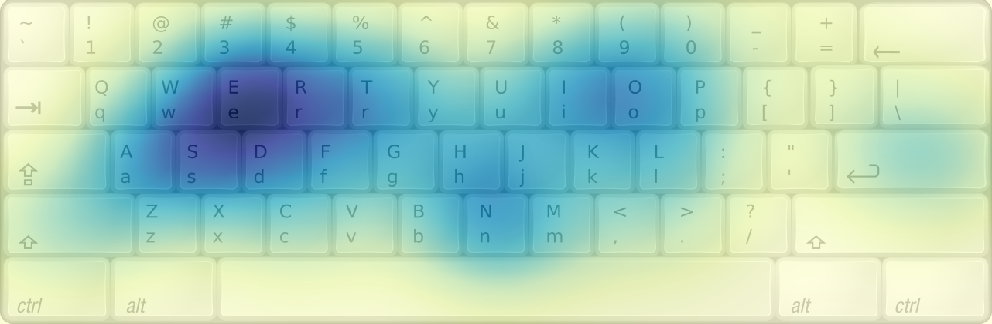
\includegraphics[width=\linewidth]{images/NoMathTxt.png}}
            \end{figure}
            %
        \end{column}
    \end{columns}
\end{frame} 
%
%
%
%
\begin{frame}{Heatmap Comparision}
    \begin{columns}
        \begin{column}{0.49\textwidth}
            \begin{figure}[h!]
                \centering
                \only<1>{\mintinline{text}|maths_heavy.tex| file \\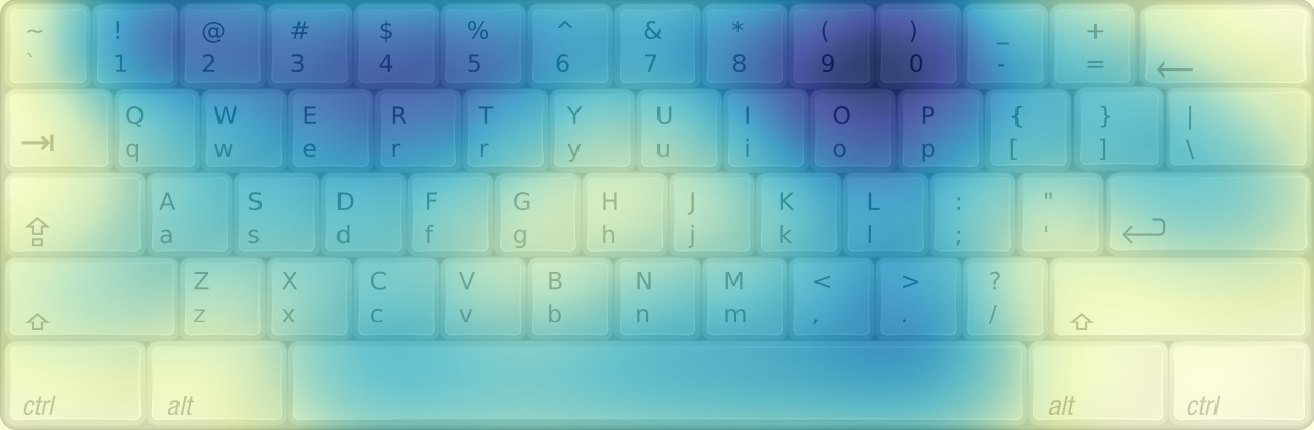
\includegraphics[width=\linewidth]{images/MathHeavyTex.png}}
                \only<1>{\mintinline{text}|maths_heavy.txt| file \\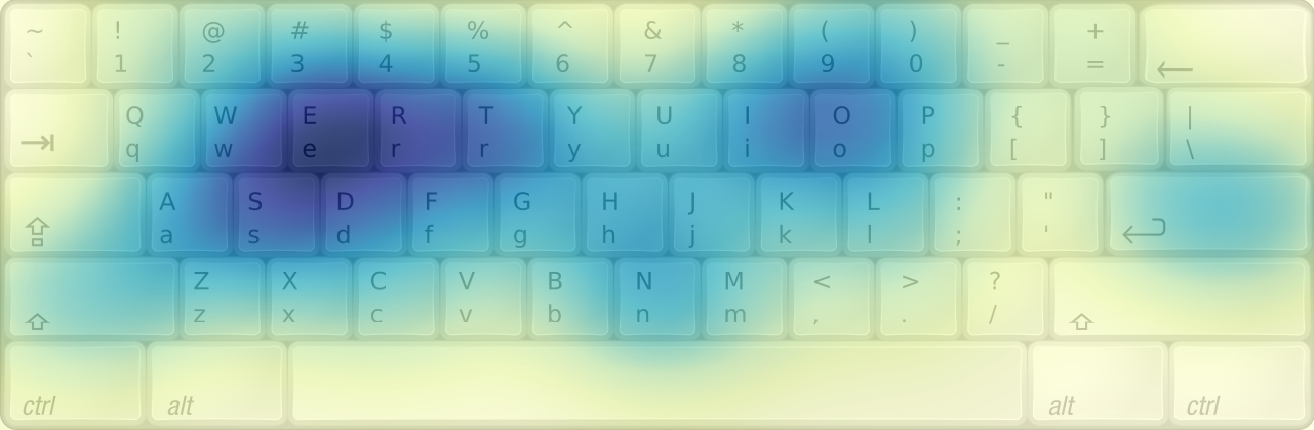
\includegraphics[width=\linewidth]{images/MathHeavyTxt.png}}
            \end{figure}
        \end{column}
        \begin{column}{0.49\textwidth}
            \begin{figure}[h!]
                \centering
                \only<1>{\mintinline{text}|text_heavy.tex| file \\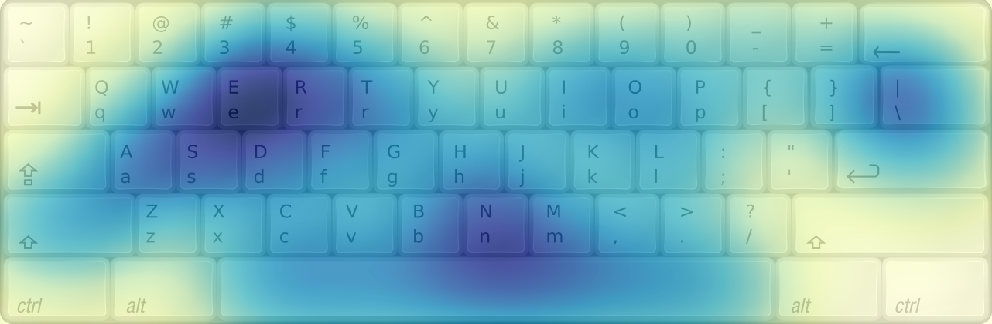
\includegraphics[width=\linewidth]{images/NoMathTex.png}}
                \only<1>{\mintinline{text}|text_heavy.txt| file \\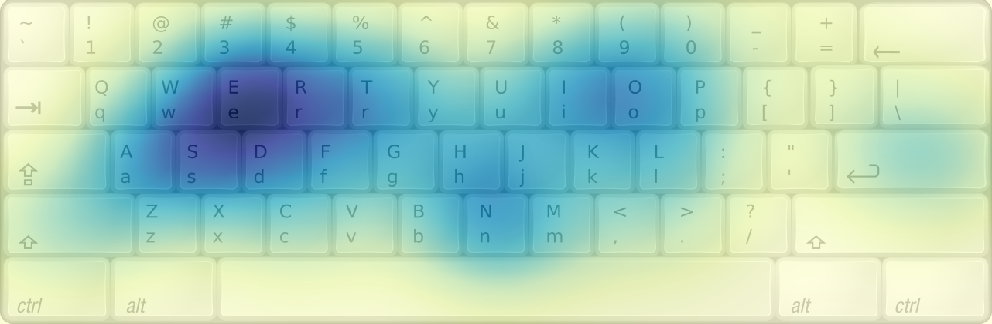
\includegraphics[width=\linewidth]{images/NoMathTxt.png}}
            \end{figure}
            %
        \end{column}
    \end{columns}
\end{frame} 
%
%
%
\begin{frame}{HeatmapGenerator}
    \begin{columns}
        \begin{column}{0.49\textwidth}
            \begin{itemize}
                \item \code[bash]{pip install kbhmap}
                \item \code[bash]{kbhmap -i <textfile> -o <imagefile>}
                \item \hspace{-2mm}\url{github.com/pranphy/KeyboardHeatmap}
            \end{itemize}
        \end{column}
        \begin{column}{0.49\textwidth}
            \vspace{-5mm} 
            \begin{figure}[h!]
                \only<1>{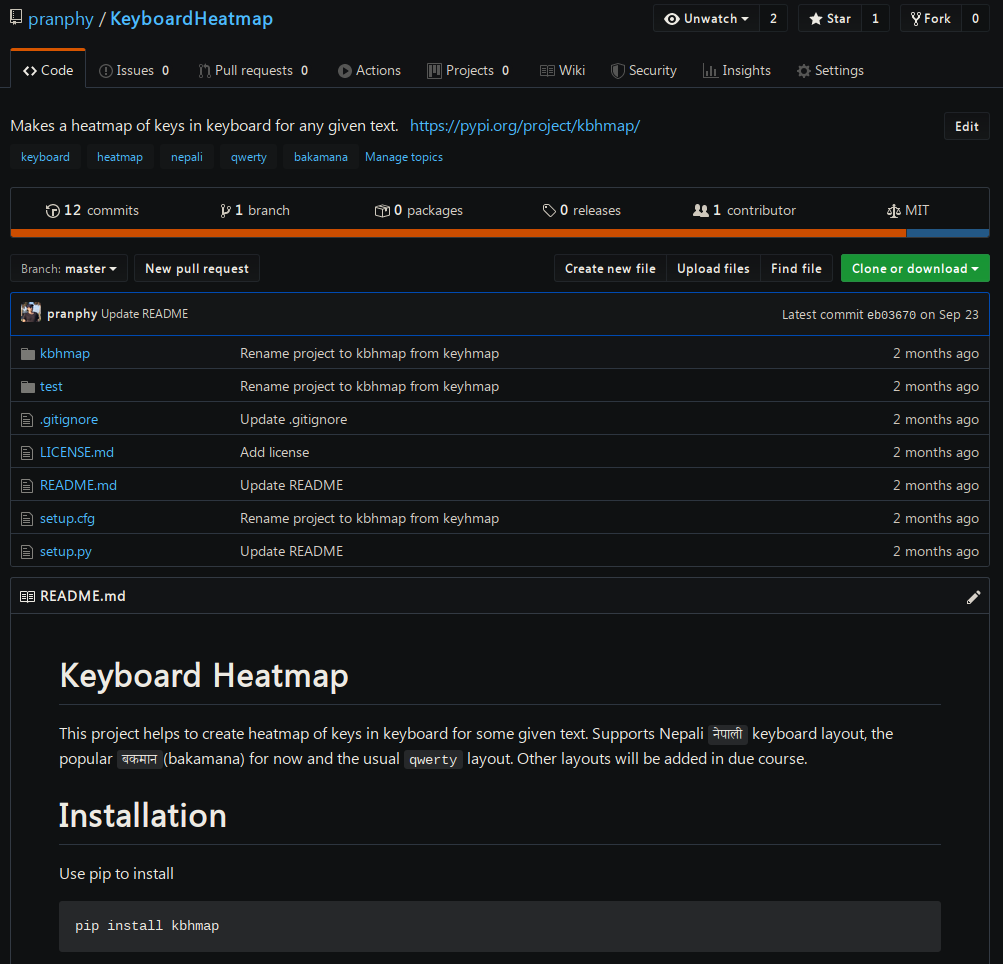
\includegraphics[width=\linewidth]{images/KeyboardHeatmapBigger.png}}
            \end{figure}
            %
        \end{column}
    \end{columns}
\end{frame} 
%
%%
%
%
\begin{frame}[fragile]{Custom Styles}
    \begin{columns}
        \begin{column}{0.39\textwidth}
            \begin{itemize}
                \item<1-> Defining own macro is a very useful tool.
                \item<1-> They can be organized into a custom \code{.sty} files and used as \mintinline{latex}|\usepackage{mystyle.sty}|
            \end{itemize}
            \begin{minted}[autogobble,fontsize=\tiny,bgcolor=cblak,breaklines=true]{latex}
                % define macro in mystyle.sty
                \newcommand{\msun}{M_{\odot}}
                \newcommand{\e}[1]{\times 10^{#1}}

                % use macro in .tex source 
                Mass of sun is $\msun = 1.9\e{30}$kg.
                % as ooposed to
                Mass of sun is $M_{\odot} = 1.9 \times 10 ^ {30}$kg
            \end{minted}
        \end{column}
        \begin{column}{0.59\textwidth}
            \begin{columns}
                \begin{column}{0.49\textwidth}
                    \only<1>{\inputminted[fontsize=\tiny,bgcolor=cblak,breaklines=true]{tex}{stycontent.tex}}
                \end{column}
                \begin{column}{0.49\textwidth}
                    \only<1>{\inputminted[fontsize=\Tiny,bgcolor=cblak]{latex}{styuse.tex}}
                \end{column}
            \end{columns}
        \end{column}
    \end{columns}
\end{frame} 
%
%
%
\begin{frame}[fragile]{Snippets (aka Lifesaver)}
    \begin{columns}
        \begin{column}{0.49\textwidth}
            \begin{itemize}
                \item Snippets are little piece of redundant code.
                \item They are easier to remember, (because you make it)
                \item They dramatically reduce the error and the speed of typesetting.
            \end{itemize}
        \end{column}
        \begin{column}{0.49\textwidth}
            \begin{minted}[autogobble,fontsize=\tiny,bgcolor=cblak]{latex}
                snippet alins " align asterisk " bA
                \begin{align*}
                    \$1
                \end{align*}
                endsnippet
            \end{minted}
            \begin{minted}[autogobble,fontsize=\tiny,bgcolor=cblak]{latex}
                snippet cases "cases from ams math" b
                \begin{cases}
                   $1 & \text{if} ${2:x\leq 0} \\\\
                   $3 & \text{if} ${4:\text{otherwise}}
                \end{cases}
                endsnippet
            \end{minted}
        \end{column}
    \end{columns}
\end{frame} 
%
%
%
\begin{frame}{Bibliography Management}
    \begin{columns}
        \begin{column}{0.49\textwidth}
            \begin{itemize}
                \item We read a lot of paper, and we need to cite them
                \item Use \mintinline{python}|.bib| file to manage bibliography.
                \item Zotero (free and Open Source) is a fantastic tool for bibliography management.
            \end{itemize}
        \end{column}
        \begin{column}{0.49\textwidth}
            %\only<1>{\inputminted[language=TeX,fontsize=\Tiny \ttfamily,bgcolor=cblak]{bibuse.tex}}
            \only<1>{\inputminted[fontsize=\tiny,bgcolor=cblak,breaklines=true]{latex}{bibuse.tex}}
        \end{column}
    \end{columns}
\end{frame} 
%
%
%
\end{document}

